\documentclass[12pt]{article}
\usepackage[utf8]{inputenc}
\usepackage{graphicx}
\usepackage{amsmath}
\usepackage{xcolor}
\usepackage{listings}
\usepackage[margin=1in]{geometry}
\usepackage{hyperref}
\usepackage{caption}
\usepackage{subcaption}
\usepackage{titlesec}
\usepackage{booktabs}
\usepackage{float}
\usepackage{afterpage}

\definecolor{codebg}{rgb}{0.95,0.95,0.95}
\definecolor{myblue}{rgb}{0,0.3,0.6}

\lstset{
    backgroundcolor=\color{codebg},
    basicstyle=\ttfamily\small,
    breaklines=true,
    frame=single,
    numbers=left,
    numberstyle=\tiny\color{gray},
    keywordstyle=\color{myblue},
    commentstyle=\color{green!50!black},
    stringstyle=\color{red},
    showstringspaces=false,
    tabsize=4
}

\title{Image Skeletonization Using Morphological Operations}
\date{\today}

\begin{document}

\maketitle

\begin{abstract}
This document demonstrates a complete image skeletonization pipeline using morphological operations. The process includes image preprocessing, edge detection, erosion/dilation, skeleton extraction, and skeleton refinement.
\end{abstract}

\section{Libraries Used}
\begin{itemize}
    \item \texttt{numpy}: For numerical operations and array manipulation
    \item \texttt{cv2} (OpenCV): For image loading and basic processing
    \item \texttt{matplotlib.pyplot}: For image visualization and plotting
\end{itemize}

\section{Step-by-Step Process}

\subsection{Step 1: Import Libraries}
\begin{lstlisting}[language=Python]
import numpy as np
import cv2 as cv
import matplotlib.pyplot as plt
\end{lstlisting}

\subsection{Step 2: Download Images}
Download sample images from GitHub repository:
\begin{lstlisting}[language=Python]
!wget https://raw.githubusercontent.com/AsadiAhmad/Image-Skeletonizer/main/Pictures/hand.jpg -O hand.jpg
!wget https://raw.githubusercontent.com/AsadiAhmad/Image-Skeletonizer/main/Pictures/shark.jpg -O shark.jpg
!wget https://raw.githubusercontent.com/AsadiAhmad/Image-Skeletonizer/main/Pictures/human.jpg -O human.jpg
!wget https://raw.githubusercontent.com/AsadiAhmad/Image-Skeletonizer/main/Pictures/cow.jpg -O cow.jpg
\end{lstlisting}

\subsection{Step 3: Load and Display Images}
Load images in grayscale and display:
\begin{lstlisting}[language=Python]
hand = cv.imread("hand.jpg", cv.IMREAD_GRAYSCALE)
shark = cv.imread("shark.jpg", cv.IMREAD_GRAYSCALE)
human = cv.imread("human.jpg", cv.IMREAD_GRAYSCALE)
cow = cv.imread("cow.jpg", cv.IMREAD_GRAYSCALE)

plt.figure(figsize=[13, 6])
plt.subplot(141),plt.imshow(hand, cmap='gray'),plt.title('hand');
plt.subplot(142),plt.imshow(shark, cmap='gray'),plt.title('shark');
plt.subplot(143),plt.imshow(human, cmap='gray'),plt.title('human');
plt.subplot(144),plt.imshow(cow, cmap='gray'),plt.title('cow');
plt.show()
\end{lstlisting}

\begin{figure}[H]
    \centering
    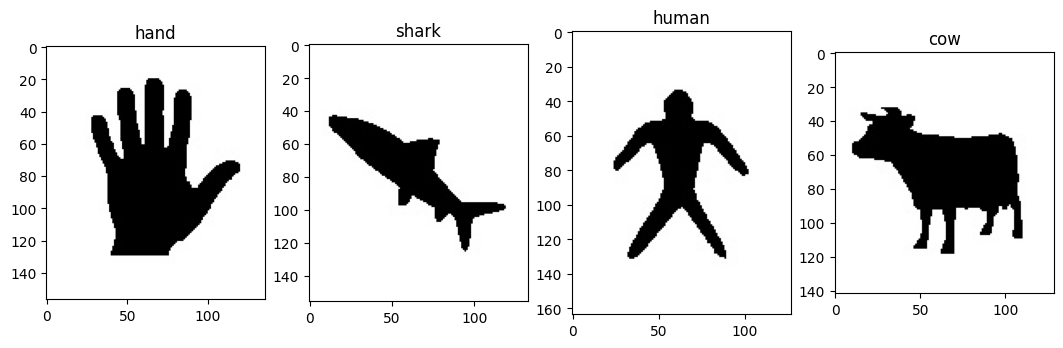
\includegraphics[width=\textwidth]{original_images.png}
    \caption{Original grayscale images}
    \label{fig:original}
\end{figure}

\subsection{Step 4: Image Inversion}
Invert images for better processing:
\begin{lstlisting}[language=Python]
hand = 255 - hand
shark = 255 - shark
human = 255 - human
cow = 255 - cow
\end{lstlisting}

\begin{figure}[H]
    \centering
    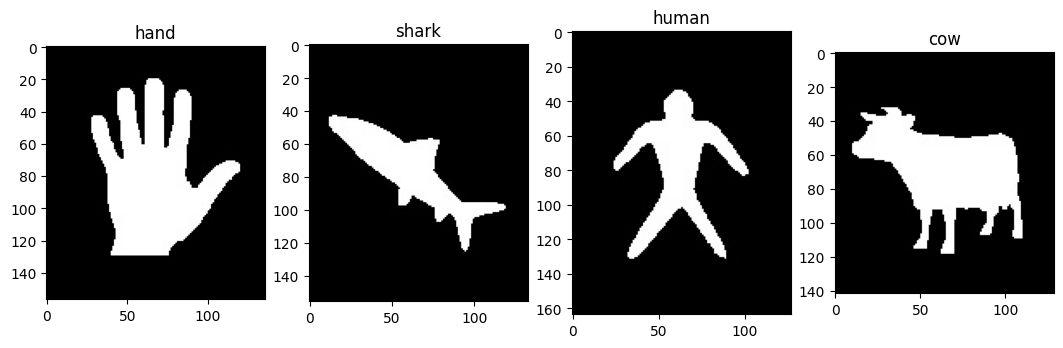
\includegraphics[width=\textwidth]{inverted_images.png}
    \caption{Inverted images}
    \label{fig:inverted}
\end{figure}

\subsection{Step 5-6: Binarization}
Convert to binary images:
\begin{lstlisting}[language=Python]
hand = np.where(hand > 127, 255, 0)
shark = np.where(shark > 127, 255, 0)
human = np.where(human > 127, 255, 0)
cow = np.where(cow > 127, 255, 0)

hand //= 255
shark //= 255
human //= 255
cow //= 255
\end{lstlisting}

\subsection{Step 7: Define Kernels}
Create morphological operation kernels:
\begin{lstlisting}[language=Python]
# Corner kernels
nw_kernel = np.array([[-1, -1,  0], [-1, 1, 1], [0, 1, 0]], dtype=np.int8)
ne_kernel = np.array([[0, -1, -1], [1, 1, -1], [0, 1, 0]], dtype=np.int8)
se_kernel = np.array([[0, 1, 0], [1, 1, -1], [0, -1, -1]], dtype=np.int8)
sw_kernel = np.array([[0, 1, 0], [-1, 1, 1], [-1, -1, 0]], dtype=np.int8)

# Edge kernels
n_kernel = np.array([[-1, -1, 0], [1, 1, 0], [0, 0, 0]], dtype=np.int8)
e_kernel = np.array([[0, 1, -1], [0, 1, -1], [0, 0, 0]], dtype=np.int8)
s_kernel = np.array([[0, 0, 0], [0, 1, 1], [0, -1, -1]], dtype=np.int8)
w_kernel = np.array([[0, 0, 0], [-1, 1, 0], [-1, 1, 0]], dtype=np.int8)

# Dilation/erosion kernels
big_kernel = np.array([[0,0,1,0,0],[0,1,1,1,0],[1,1,1,1,1],
                      [0,1,1,1,0],[0,0,1,0,0]], dtype=np.uint8)
small_kernel = np.ones((3,3), dtype=np.uint8)
\end{lstlisting}

\subsection{Step 8-9: Edge Detection}
Implement hit-or-miss edge detection:
\begin{lstlisting}[language=Python]
def calculate_hit_or_miss(image, kernel, condition_sum):
    converted_image = np.where(image == 1, 1, -1).astype(np.int8)
    height, width = converted_image.shape
    matrix = np.zeros((height, width), dtype='int8')
    for i in range(1, height-2):
        for j in range(1, width-2):
            result = converted_image[i-1:i+2, j-1:j+2] * kernel
            if sum(result.flatten()) == condition_sum:
                matrix[i, j] = 1
    return matrix

def edge_detection(image):
    matrices = [calculate_hit_or_miss(image, k, c) 
               for k, c in zip([nw_kernel, ne_kernel, sw_kernel, se_kernel,
                               n_kernel, e_kernel, s_kernel, w_kernel],
                              [6,6,6,6,4,4,4,4])]
    final_matrix = matrices[0].copy()
    for mat in matrices[1:]:
        final_matrix = np.logical_or(final_matrix, mat)
    return final_matrix.astype(np.int8)

edge_hand = edge_detection(hand)
\end{lstlisting}

\begin{figure}[H]
    \centering
    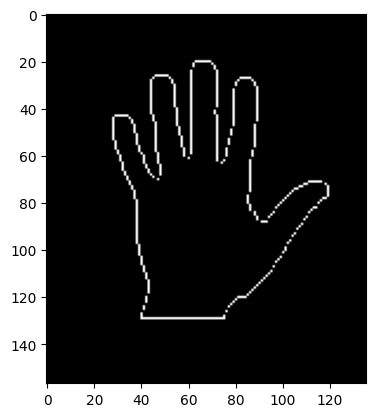
\includegraphics[width=0.5\textwidth]{edge_detection.png}
    \caption{Edge detection result}
    \label{fig:edge}
\end{figure}

\subsection{Step 10: Erosion Operation}
Erosion is a morphological operation that shrinks foreground regions. A pixel is set to 1 only if all kernel elements match the corresponding image pixels:
\begin{lstlisting}[language=Python]
def calculate_erosion(image, kernel):
    condition_sum = np.count_nonzero(kernel)
    height, width = image.shape
    pad = kernel.shape[0]//2
    result = np.zeros_like(image)
    for i in range(pad, height-pad):
        for j in range(pad, width-pad):
            if (image[i-pad:i+pad+1, j-pad:j+pad+1]*kernel).sum() == condition_sum:
                result[i,j] = 1
    return result
\end{lstlisting}

\begin{figure}[H]
    \centering
    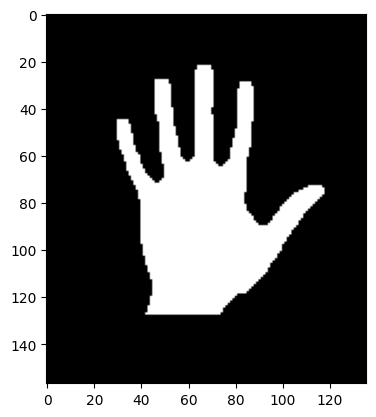
\includegraphics[width=0.4\textwidth]{erosion.png}
    \caption{Erosion result showing thinning of foreground regions}
    \label{fig:erosion}
\end{figure}

\subsection{Step 11: Dilation Operation}
Dilation expands foreground regions. A pixel is set to 1 if any kernel element matches a corresponding image pixel:
\begin{lstlisting}[language=Python]
def calculate_dilation(image, kernel):
    pad = kernel.shape[0]//2
    height, width = image.shape
    result = np.zeros_like(image)
    for i in range(pad, height-pad):
        for j in range(pad, width-pad):
            if (image[i-pad:i+pad+1, j-pad:j+pad+1]*kernel).any():
                result[i,j] = 1
    return result
\end{lstlisting}

\begin{figure}[H]
    \centering
    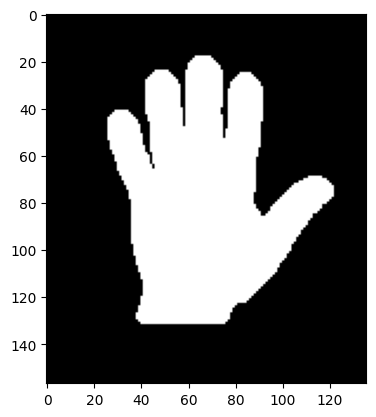
\includegraphics[width=0.4\textwidth]{dilation.png}
    \caption{Dilation result showing expansion of foreground regions}
    \label{fig:dilation}
\end{figure}

\subsection{Step 12: Skeletonization}
Extract image skeletons:
\begin{lstlisting}[language=Python]
def calculate_skeleton(image, kernel, iterations=18):
    skeleton_parts = []
    current = image.copy()
    for _ in range(iterations):
        eroded = calculate_erosion(current, kernel)
        skeleton_parts.append(edge_detection(current))
        current = eroded
        if not current.any(): break
    skeleton = skeleton_parts[0]
    for part in skeleton_parts[1:]:
        skeleton = np.logical_or(skeleton, part)
    return skeleton.astype(np.uint8)

hand_skeleton = calculate_skeleton(hand, big_kernel)
\end{lstlisting}

\begin{figure}[H]
    \centering
    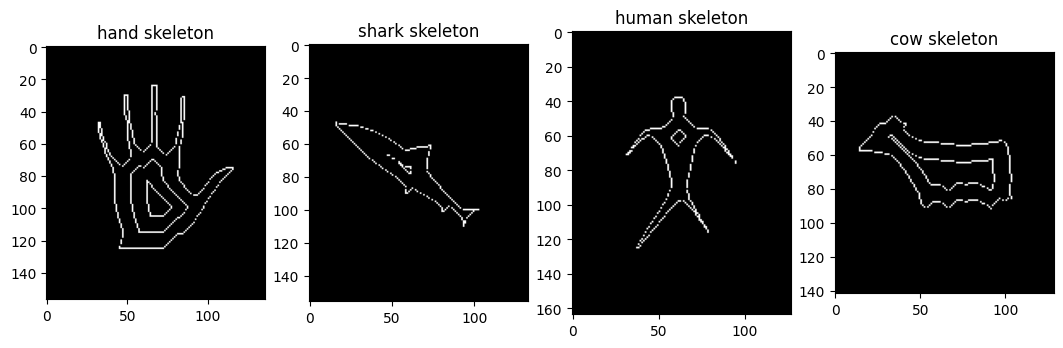
\includegraphics[width=\textwidth]{skeletons.png}
    \caption{Skeletonization results for all images}
    \label{fig:skeletons}
\end{figure}

\subsection{Step 13-16: Skeleton Refinement}
Refill and finalize skeletons:
\begin{lstlisting}[language=Python]
def refill_skeleton(skeleton, big_kernel, small_kernel):
    dilated = calculate_dilation(skeleton, big_kernel)
    dilated = calculate_dilation(dilated, big_kernel)
    return calculate_dilation(dilated, small_kernel)

hand_filled = 255 - (refill_skeleton(hand_skeleton, big_kernel, small_kernel) * 255)
\end{lstlisting}

\begin{figure}[H]
    \centering
    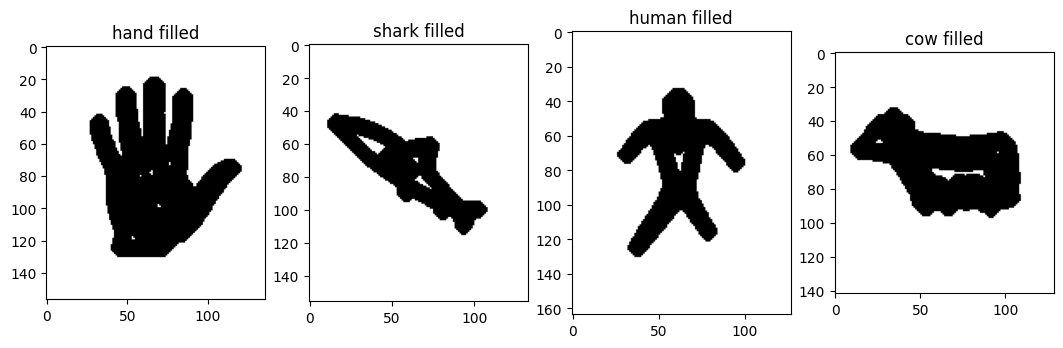
\includegraphics[width=\textwidth]{final_results.png}
    \caption{Final refilled skeleton results}
    \label{fig:final}
\end{figure}

\section{Technical Explanations}

\subsection{Morphological Operations}
\begin{itemize}
    \item \textbf{Erosion}: Shrinks objects by removing boundary pixels
    \item \textbf{Dilation}: Expands objects by adding pixels to boundaries
    \item \textbf{Skeletonization}: Reduces objects to 1-pixel wide representations
    \item \textbf{Hit-or-Miss}: Detects specific patterns in binary images
\end{itemize}

\begin{center}
    \href{https://github.com/AsadiAhmad/Image-Skeletonizer}{
        \includegraphics[width=0.2\textwidth]{github_logo.png} \\
        \texttt{https://github.com/AsadiAhmad/Image-Skeletonizer}
    }
\end{center}

\end{document}